\section{The Large Hadron Collider}
\label{sec:Det:LHC}

The Large Hadron Collider (LHC) is situated 100m below the border between Switzerland and France near the Swiss city of Geneva. 
The LHC was designed to provide two proton beams with 2808 bunches in each beam colliding with 25 ns bunch spacing at a centre-of-mass energy of 14TeV.
Around the LHC ring, which is 26.6km long, there are four interaction points. 
The four experiments at these interaction points are ATLAS, CMS, LHCb and ALICE.
ATLAS and CMS are general purpose detectors designed to be able to detect a broad range of physics. ALICE is designed to investigate heavy ion collisions, and LHCb is designed to explore CP violation and rare b-decays.
Figure \ref{Det:LHC} shows the layout of the LHC, and the four experiments.

\begin{figure}
\centering
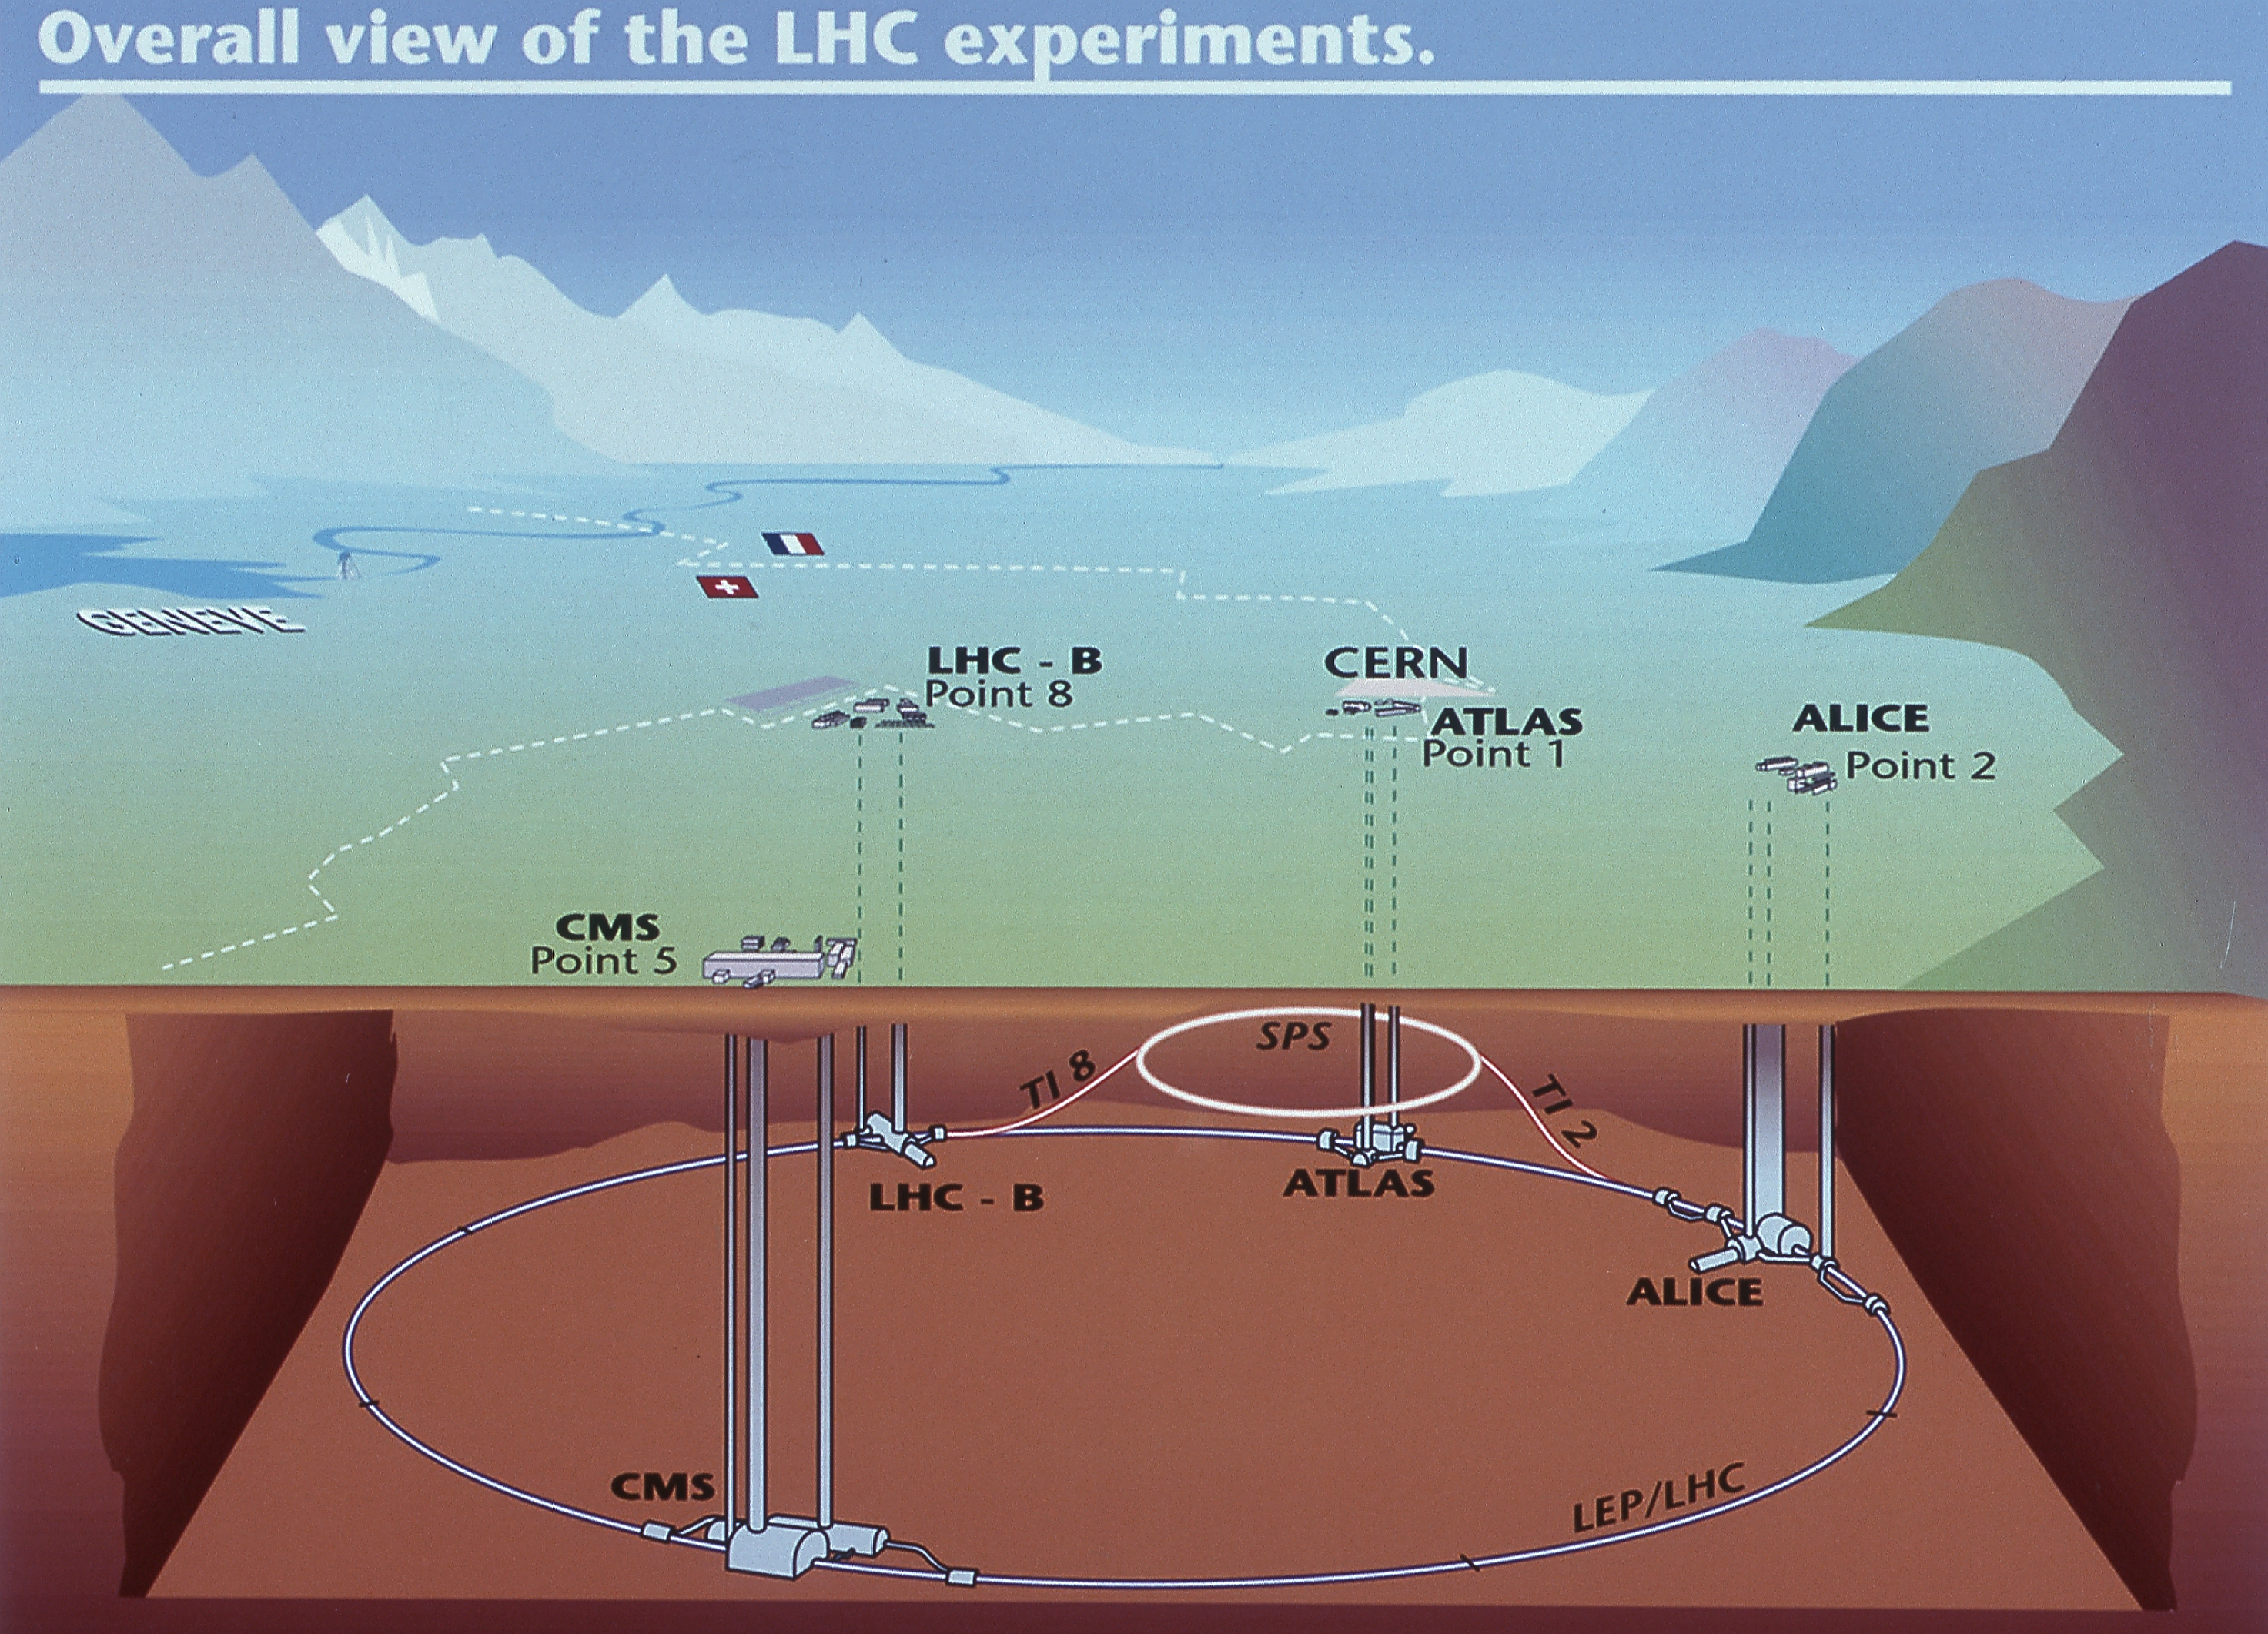
\includegraphics[width=0.9\textwidth]{figures/Detector/AtlasSite.jpg}
  \caption{The LHC and the sites of the 4 main LHC experiments.}
\label{Det:LHC}
\end{figure}

A series of accelerators provide proton bunches to the LHC at an energy of 450 GeV.
The proton bunches are then accelerated around the LHC by an array of superconducting dipole magnets to provide a beam energy up to 7 TeV.


\subsection{Luminosity}

The event rate of a process X is
\begin{equation}
R_X = L \sigma_X,
\label{Det:Lumi}
\end{equation}
where $\sigma_X$ is the cross section for the process and L is the luminosity.

Achieving a large luminosity is important for observing physics processes that have a low cross-section, and an accurate luminosity determination is important for measuring differential cross-sections of processes from the event rate. 

Luminosity is defined by,
\begin{equation}
L=\frac{N_b^2n_bf_{rev}\gamma_r}{4\pi\epsilon_n\beta^\star}F
\label{Det:Lumi}
\end{equation}
where $N_b$ is the number of particles per bunch, $n_b$ is the number of colliding bunches per beam, $f_{rev}$ is the revolution frequency, $\gamma_r$ is the relativistic gamma factor, $\epsilon_n$ is the normalised transverse beam emitance, $\beta^\star$ is the $\beta$ function at the interaction point, and $F$ is the geometric luminosity reduction factor due to the crossing angle of the beams.


Equation \ref{Det:Lumi} is useful to understand both the luminosity and how to increase it. 
However, the beam current changes throughout a run, so the equation is not ideal to measure the luminosity during a run.
*I am ot sure this is the only reason, it may also be due to the precision of the beam current measurement* 
An alternative way of acquiring the instantaneous luminosity is to measure the interaction rate via various ATLAS detectors and correlate this to the luminosity. 
The interaction rate is either the hit rate or the event rate for a given detector.
The luminosity defined by the interaction rate is,
\begin{equation}
L=\frac{\mu n_bf_{rev}}{\sigma_{inel}}=\frac{\mu_{vis}n_bf_{rev}}{\sigma_{vis}}
\label{Det:Lumi2}
\end{equation}
where $\mu$ is the number of inelastic collisions per bunch crossing, $\sigma_{inel}$ is the inelastic cross-section, $\mu_{vis}$ is the number of visible inelastic collisions per bunch crossing, and $\sigma_{vis}$ is visible inelastic cross-section. 


The calibration constant that associates the luminosity to the $\mu_{vis}$, which is measured using interaction rates, is $\sigma_{vis}$.
One method of obtaining the calibration constant $\sigma_{vis}$, and thus the absolute luminosity, is using a van der Meer scan method.
The method aims to measure the interaction rate when the two beams are perfectly aligned, while also measuring the beam currents.
This is achieved by scanning one beam over the other in the x-y plane. 
The interaction rate is fitted as a function of separation in x and y separately, and the maximum interaction rate is found at the peak of each fit. 
The 2010 data luminosity calibrated by the van der Meer scan method has a luminosity uncertainty of 3.4\%.

The amount of data that an experiment collects is expressed using the integrated luminosity, which is the integral over time of the luminosity.

\subsubsection{2010 run}
The 7 TeV centre-of-mass proton-proton run in 2010 was the first substantial data-taking period provided by the LHC. 
The initial runs provided peak luminosity of \lumi{\sim0.01\times10^{30}} from one pair of interacting bunches with a very low number of protons per bunch. 
By the end of the 2010 data-taking run the peak luminosity was \lumi{\sim2\times10^{32}} from 348 colliding bunches.
The luminosity increase was mainly achieved by increasing the number of colliding bunches per beam and the number of protons per bunch, though decreasing the $\beta^\star$ and reducing the beams crossing angle also increased the luminosity.


The 2010 data taking run was split into different data periods, where a new period would be started when there was a significant change in the beam parameters.
Table \ref{Det:Periods} shows the data periods for the 2010 LHC run, and how the beam conditions and peak luminosity changed.  
Additionally, periods G-I had used bunch trains where bunches were grouped together with 150 ns spacing between the bunches.  


The total integrated luminosity delivered by the LHC for the 2010 run was 48.1 $pb^1$.

\begin{table}
\begin{center}
\begin{tabular}{|c|c|c|c|c|}
\hline
Period&Date&Peak Luminosity& $N_b$ & $n_b$ \\
& &\lumi{}& $\times10^{11}$ & \\
\hline
A & Mar 30 - Apr 18 & 0.004 & <0.01 & 1 \\
B & Apr 23 - May 17 & 0.06 & 0.01-0.6 & 1-3 \\
C & May 18 - June 5 & 0.2 & 0.7-1.9 & 3-8 \\
D & June 18 - July 19 & 1.6 & 3-8 & 2-8 \\
E & July 29 - Aug 18 & 3.9 & 12-14 & 16 \\
F & Aug 19 - Aug 30 & 10 & 35-100 & 32-36 \\
G & Sept 22 - Oct 7 & 70 & 100-200 & 50-186 \\
H & Oct 8 - Oct 18 & 150 & 250-350 & 233-300 \\
I & Oct 24 - Oct 29 & 210 & 350-400 & 300-350 \\
\hline
\end{tabular}
\caption{ Beam information for the different data taking periods.}
\label{Det:Periods}
\end{center}
\end{table}

